\documentclass{article}

\usepackage{a4}
\usepackage{amsmath}
\usepackage{amssymb}
\usepackage{ctex}
\usepackage{booktabs}
\usepackage{graphicx}
\usepackage{float}
\usepackage{hyperref}
\usepackage{enumitem}
\usepackage{array}
\usepackage{fvextra}
\usepackage{xurl}

\hypersetup{colorlinks=true,linkcolor=black,urlcolor=blue,citecolor=black}
\RecustomVerbatimEnvironment{verbatim}{Verbatim}{
  breaklines=true,
  breakanywhere=true,
  fontsize=\small
}
\newcommand{\TraceSize}{\fontsize{5}{6.05}\selectfont}
\newcommand{\tracecol}[2]{%
  \begin{minipage}[t]{0.492\textwidth}
    \centering{\small #1}\par\vspace{0.25em}
    \VerbatimInput[fontsize=\TraceSize,breaklines=true,breakanywhere=true]{#2}
  \end{minipage}%
}
\newcommand{\tracepair}[2]{%
  \par\noindent\tracecol{gettrace}{#1}\hfill\tracecol{mycpu}{#2}\par
}
\setlist[itemize]{nosep,leftmargin=1.8em}
\setlist[enumerate]{nosep,leftmargin=1.8em}

\title{计算机体系结构\\实验3\\异常与中断的添加}
\author{鲁昕宁 \quad 2414015}
\date{2026年11月10日}
\begin{document}

\maketitle
\begin{center}
\begin{tabular}{ll}
GitHub仓库 & \parbox[t]{0.72\textwidth}{\url{SidneyLu/Computer-Architecture-NKU-CS/tree/master/lab3}} \\[0.6em]
班号 & \underline{0964} \\[0.6em]
授课教师 & \underline{董前琨} \\[0.6em]
\end{tabular}
\end{center}

\newpage

\section{实验目标}
本实验接着实验2的五级流水线，完成《CPU设计实战》第7章两个实践任务。
CPU 仍是 \texttt{mycpu\_verify/rtl/myCPU}。

\begin{enumerate}
  \item 增加 \texttt{MFC0}、\texttt{MTC0}、\texttt{ERET} 和 \texttt{SYSCALL}，
        以及 CP0 的 Status、Cause、EPC，使 \texttt{func\_lab8} 的 69 个功能点与参考轨迹一致。
  \item 增加 Break、地址错、整数溢出和保留指令，以及 Count、Compare、BadVAddr。
        定时器中断固定在硬件中断 5，即 Cause 的 IP7。
        硬件中断 0～5 对应 IP7～IP2，软件中断对应 IP1、IP0。
        \texttt{func\_lab9} 共 94 个功能点。
\end{enumerate}

前递、load-use 停顿、HI/LO 和延迟槽沿用实验1、实验2。
实验箱未接，比特流没有下载。
\texttt{func\_lab8}、\texttt{func\_lab9} 的轨迹对比之外，另有一段定向程序把
SYSCALL、其余异常和三种中断的 Cause、EPC 记下来并画出波形。
记忆游戏用官方二进制在仿真里走完一轮。

\section{实验原理}
异常和中断都在写回级写入 CP0。写回之前的三级只负责判定，并把 BD、异常有效位、
ExcCode、CP0 操作和 BadVAddr 随指令往后传。中断的 ExcCode 是 0，
和“没有异常”无法用编码本身区分，所以总线上单独有一位 \texttt{ex}。

\begin{center}
\begin{tabular}{lp{0.72\textwidth}}
\toprule
流水级 & 本级负责的事 \\
\midrule
译码 & \texttt{SYSCALL}、\texttt{BREAK}、保留指令、取指地址错；标记延迟槽；
       给 \texttt{ADD}/\texttt{ADDI}/\texttt{SUB} 带上溢出检查 \\
执行 & 有符号溢出、读写地址错；置 \texttt{ex\_cancel}，关掉数据 RAM 写使能 \\
访存 & 把异常信息、\texttt{rt} 和 BadVAddr 交给写回；地址错的 load 不再产生写回数据 \\
写回 & 更新 CP0，响应中断，清空流水线；\texttt{MFC0} 在这里读出 CP0 \\
\bottomrule
\end{tabular}
\end{center}

\subsection{CP0}
CP0 是写回级里的一组寄存器，布局按参考 CPU 的 GS132，
因为 trace 比较的是 \texttt{MFC0} 写出的 32 位，处理程序后来做的掩码不影响这次比较。

复位时 Status 为 \texttt{0x10400004}：CU0（位 28）、BEV（位 22）、ERL（位 2）为 1。
Cause 的 ExcCode 复位为 \texttt{0x1f}，其余位为 0。
BEV 为 1 时异常入口是 \texttt{0xbfc00380}，否则是 \texttt{0x80000180}。
测试在进入异常前执行 \texttt{mtc0}，把 Status 写成 \texttt{0x00400000}。
这次写入留下 BEV，清掉 ERL、EXL 和 IE，入口仍是 \texttt{0xbfc00380}。

\texttt{MTC0} 写 Status 时只改这些位：CU0、BEV、NMI、IM7～IM0、KSU、ERL、EXL、IE。
异常写入 CP0 时把 EXL（位 1）置 1，因此 \texttt{SYSCALL} 之后 Status 变成
\texttt{0x00400002}。\texttt{ERET} 总是清 ERL；ERL 为 0 时同时清 EXL。
同一拍里异常优先于 \texttt{ERET}，\texttt{ERET} 又优先于 \texttt{MTC0} 对 EXL、ERL 的修改。

EPC 和 Cause.BD 只在把异常写入 CP0、且当时 EXL 为 0 时更新。
发生异常的指令带 BD 时，EPC 等于它的 PC 减 4，否则 EPC 就是它的 PC。
EXL 已经为 1 时再进入异常，只改 ExcCode，EPC 保持不变。
处理程序里的 \texttt{MTC0} 写 EPC 本身不是异常，用来把返回地址改成加 4 或加 8 之后的值。

Cause 按 MIPS 的域拼出来：位 31 是 BD，位 30 是 TI，位 15～8 是 IP7～IP0，
位 6～2 是 ExcCode。CE、DC、IV 等本实验用不到的域保持 0。
\texttt{MFC0} 可读的号是 8、9、11、12、13、14，对应 BadVAddr、Count、Compare、
Status、Cause、EPC，其它号返回 0。

\begin{center}
\begin{tabular}{ll}
\toprule
来源 & ExcCode \\
\midrule
中断 & 0 \\
取指地址错、load 地址错（AdEL） & 4 \\
store 地址错（AdES） & 5 \\
\texttt{SYSCALL} & 8 \\
\texttt{BREAK} & 9 \\
保留指令 & 10 \\
\texttt{ADD}/\texttt{ADDI}/\texttt{SUB} 溢出 & 12 \\
\bottomrule
\end{tabular}
\end{center}

\subsection{各类异常怎么判定}
指令编码和 PC 在译码级已经齐全，下面几类在这里确定。

\begin{itemize}
  \item \texttt{SYSCALL}、\texttt{BREAK} 是特殊指令功能码 \texttt{0x0c}、\texttt{0x0d}。
        它们不写通用寄存器。
  \item 保留指令：操作码不属于实验2已经实现的集合，也不是
        \texttt{MFC0}、\texttt{MTC0}、\texttt{ERET}。取指地址错优先于保留指令，
        避免把一个错地址上读来的字再当成非法操作码。
  \item 取指地址错：该指令的 PC 最低两位不是 0。BadVAddr 记这个 PC。
        同时把访存操作、乘除操作和寄存器写使能清掉，分支也不采纳，
        这样错地址上读到的编码不会去写 HI/LO 或改 PC。
\end{itemize}

执行级能看到 ALU 结果之后再补两类。译码级已经判定为异常的指令保持原来的 ExcCode。

\begin{itemize}
  \item 溢出只检查 \texttt{ADD}、\texttt{ADDI}、\texttt{SUB}。
        加法在两个操作数符号相同、结果符号与它们不同时溢出。
        减法在两个操作数符号不同、结果符号与被减数不同时溢出。
        \texttt{ADDU}、\texttt{ADDIU}、\texttt{SUBU} 不检查。
        溢出的算术指令译码时本来会写寄存器，写回级看到异常后把 \texttt{rf\_we} 拉低，
        目的寄存器保持进入异常之前的值。
  \item \texttt{LW}、\texttt{SW} 在地址最低两位非 0 时分别是 AdEL、AdES。
        \texttt{LH}、\texttt{LHU}、\texttt{SH} 只看最低一位。
        \texttt{LB}、\texttt{LBU}、\texttt{SB} 以及 \texttt{LWL}/\texttt{LWR}/\texttt{SWL}/\texttt{SWR}
        允许任意字节对齐。访存地址错的 BadVAddr 是 ALU 算出的地址，数据 RAM 写使能为 0。
\end{itemize}

\subsection{精确异常}
若只在写回级才清空流水线，\texttt{SYSCALL} 进入写回时，后面的 \texttt{sw} 已经到达执行级，
数据 RAM 的写使能会在流水线被清空之前生效。
因此异常指令一进入执行级就产生 \texttt{ex\_cancel}。
还在取指或译码、排在它后面的指令被清成无效，新的译码结果也不能进入执行级。
\texttt{ERET} 同样拉高 \texttt{ex\_cancel}，它后面的指令不会在返回之前执行。

以 \texttt{syscall} 后跟 \texttt{sw} 为例。\texttt{syscall} 在译码级时，\texttt{sw} 还在取指。
下一拍 \texttt{syscall} 进入执行级，\texttt{ex\_cancel} 为 1，\texttt{sw} 停在译码级且不能前进，
这一拍结束时译码和取指的有效位被清掉。\texttt{syscall} 再经访存进入写回，
这一拍更新 EPC、ExcCode 和 EXL，并清空流水线。\texttt{sw} 没有到过执行级，写使能也没有打开。
处理程序返回后，这条 \texttt{sw} 会重新取指再执行，只是不能先于处理程序写回。

清空流水线时的目标地址由写回级给出：\texttt{ERET} 用当前 EPC，其它异常和中断用入口地址。
指令 RAM 的数据晚一拍返回。清空的这一拍就把这个地址送到 \texttt{inst\_sram\_addr}，
同时把取指 PC 设成同一地址、有效位置 1。下一拍读回的指令和这个 PC 配对，
第一条进入译码的就是入口上的 \texttt{mfhi}。

写回级清空流水线时还会清掉执行级和访存级。中断在写回级才决定，被打断的指令后面的 store
可能正停在执行级；写使能同时被 \texttt{wb\_flush} 掩掉，这一拍不会写入数据 RAM。
执行级里尚未写完的乘除在这时丢掉进行中的状态，HI/LO 保持原值。

\subsection{延迟槽}
译码级当前指令是分支或跳转（不论是否发生转移）时，取指级正在取的下一条就是延迟槽。
取指总线的最高位带上这个标记，该指令进入译码后成为它的 BD，再随流水线到达写回。
延迟槽中的异常写入 CP0 时，EPC 写成 BD 所指示的分支 PC。

通用处理程序读 Cause 的位 31。该位为 0 时把 EPC 加 4，否则再加 4，然后 \texttt{MTC0} 写回并 \texttt{ERET}。
普通异常因此返回到发生异常那条指令的下一条；延迟槽中的异常返回到分支后面的第二条，槽内指令不会再次执行。
\texttt{n83} 到 \texttt{n94} 把 \texttt{SYSCALL}、\texttt{BREAK}、溢出等放进
\texttt{BEQ} 到 \texttt{JALR} 的延迟槽，检查的就是这条 EPC。

\subsection{中断}
中断请求为
\begin{verbatim}
int_req = IE && !EXL && !ERL && |(Status[15:8] & IP[7:0])
\end{verbatim}
Status 位 15～8 是 IM7～IM0，与 Cause 的 IP7～IP0 按位对应。
请求在写回级采样。当前指令自身已是异常时，优先把该异常写入 CP0；
否则在 \texttt{int\_req} 为 1 时，把这条正在写回的指令当作被中断打断的指令，ExcCode 记 0。
这条指令的通用寄存器写回仍然完成，EPC 指向它。
EXL 在同一拍置 1，下一拍起 \texttt{int\_req} 为 0，处理程序执行期间不再采样新的中断。

Count 每拍翻转一位使能，使能为 1 的那一拍才加 1，和参考 CPU 的 \texttt{count\_add\_en} 相同。
\texttt{MTC0} 写 Count 的那一拍用写入值代替自增。
Count 与 Compare 相等时 TI 置 1；\texttt{MTC0} 写 Compare 的那一拍把 TI 清 0，并更新 Compare。

IP7～IP2 比中断源晚一拍写入 Cause。IP7 是外部硬件中断 5 与 TI 相或，
IP6～IP2 分别是硬件中断 4～0。IP1、IP0 只由 \texttt{MTC0} 写 Cause 的位 9、位 8。
SoC 把 \texttt{hw\_int[5:0]} 接成 0，因此 \texttt{func\_lab9} 里 IP7 只由定时器抬起。
定时器测试把 IE 和全部 IM 打开，把 Count 设到 Compare 附近，然后执行
\texttt{1: b 1b; nop}。软件中断测试用同样的 Status，再 \texttt{MTC0} 把 IP1 或 IP0 写成 1。

中断处理程序要求 EPC 等于标号 \texttt{1}，然后自己把 EPC 加 8 再 \texttt{ERET}，
从而跳过这条分支和它的延迟槽。被打断的是这条分支时，BD 为 0，EPC 就是分支 PC。
被打断的是槽里的 \texttt{nop} 时，BD 为 1，EPC 仍是分支 PC。
两条路径的返回地址相同。处理程序在读 Cause 时关闭 trace 比较，BD 的差别不会进入 \texttt{golden\_trace.txt}。

\subsection{MFC0 的数据相关}
\texttt{MFC0} 的目的寄存器是 \texttt{rt}，数值要等写回级按 \texttt{rd} 读 CP0 才存在。
执行级和访存级里的 ALU 结果不能前递。要用这个结果的指令还在译码级、而 \texttt{MFC0} 还在执行级或访存级时，
按 load-use 的条件把 \texttt{ds\_ready\_go} 拉低，译码级停两拍。
\texttt{MFC0} 到达写回后，\texttt{rf\_wdata} 换成 CP0 读数，实验1的写回前递把这个数送给下一条。
入口处理程序的典型序列是 \texttt{mfc0 k0} 紧接 \texttt{bne k0, ...}，
比较用的就是这一路前递。

\section{实验过程}
\subsection{程序与轨迹}
\texttt{func\_lab8}、\texttt{func\_lab9} 放在 \texttt{CPU\_CDE/soft/}，与 \texttt{func\_lab7} 同级。
两个工程里的 \texttt{inst\_ram} 都是锁定的旧 IP，先 \texttt{upgrade\_ip}，
再把 COE 指到对应的 \texttt{obj/inst\_ram.coe} 并重新生成仿真文件。
\texttt{cpu132\_gettrace} 跑完得到 \texttt{golden\_trace.txt}，
\texttt{mycpu} 的 testbench 在写非 0 寄存器时逐条比较。

\texttt{func\_lab8} 的测试数为 $23+19+26+1=69$，新增的一点是 \texttt{SYSCALL}。
\texttt{func\_lab9} 再加 25 点，共 94。新增点依次是 Break，
\texttt{ADD}/\texttt{ADDI}/\texttt{SUB} 溢出，
\texttt{LW}/\texttt{LH}/\texttt{LHU} 读地址错，\texttt{SW}/\texttt{SH} 写地址错，
取指地址错，保留指令，定时器中断，软件中断，
以及放在 \texttt{BEQ} 到 \texttt{JALR} 延迟槽里的异常。

\subsection{func\_lab8}
{\sloppy
69 个功能点一次通过。
第 42 点 \texttt{mycpu} 为 1077305\,ns，\texttt{gettrace} 为 1193795\,ns。
第 68 点分别为 1644675\,ns 和 1835425\,ns。
这两个时刻与实验2的 \texttt{func\_lab6}、\texttt{func\_lab7} 相同。
\par}
第 69 点是新增的 \texttt{SYSCALL}。
\texttt{mycpu} 的通过时刻是 1649965\,ns。
\texttt{gettrace} 的通过时刻是 1841065\,ns。
结束时间见第~\ref{sec:trace}~节。

\subsection{func\_lab9}
换成 \texttt{func\_lab9} 的 COE 后，前 69 点的通过时刻与 \texttt{func\_lab8} 相同。
第 70 到 94 点覆盖其余异常和中断，也全部通过。
第 94 点 \texttt{mycpu} 为 1939805\,ns，\texttt{gettrace} 为 2130615\,ns。
从第 69 点到第 94 点，两边各增加约 0.290\,ms。

\section{关键代码}
\subsection{译码级}
\texttt{inst\_known} 是实验2全部指令再加上三条 CP0 指令、\texttt{SYSCALL} 和 \texttt{BREAK} 的或。
取指地址错单独判定，排在保留指令之前。溢出检查先做成一位，随指令进入执行级。
\begin{verbatim}
wire inst_adel_if = |ds_pc[1:0];
wire inst_ri      = ~inst_known & ~inst_adel_if;
wire ds_ex        = inst_syscall | inst_break | inst_ri | inst_adel_if;
wire [4:0] ds_excode = inst_adel_if ? `EXC_ADEL :
                       inst_syscall ? `EXC_SYS  :
                       inst_break   ? `EXC_BP   :
                       inst_ri      ? `EXC_RI   : 5'd0;
wire ds_ov_en   = inst_add | inst_addi | inst_sub;
wire ds_badv_we = inst_adel_if;
\end{verbatim}
\texttt{ds\_ex} 为 1 时，送到执行级的访存操作和乘除操作都改成空操作。
保留指令的功能码即使碰巧等于 \texttt{DIV}，也不会把执行级停在除法器上。

\subsection{执行级}
\texttt{es\_alu\_op[1]} 为 1 表示减法。译码级已经判定的异常放在 \texttt{es\_ex} 里，
溢出和访存地址错只在它为 0 时生效，最后合成 \texttt{es\_ex\_f}。
\begin{verbatim}
wire es_ov = es_ov_en && (es_alu_op[1]
             ? (es_alu_src1[31] != es_alu_src2[31])
               && (alu_result[31] != es_alu_src1[31])
             : (es_alu_src1[31] == es_alu_src2[31])
               && (alu_result[31] != es_alu_src1[31]));
wire es_ex_f = es_ex || es_ov || es_adel_m || es_ades_m;
assign ex_cancel = es_valid && (es_ex_f || es_cp0_op == `CP0_ERET);
assign data_sram_wen =
    (es_valid && !wb_flush && !es_ex_f) ? st_wen : 4'h0;
\end{verbatim}
\texttt{es\_adel\_m}、\texttt{es\_ades\_m} 按上一节的对齐规则产生。
它们把 BadVAddr 改成 \texttt{alu\_result}；取指地址错则继续使用译码级传来的 PC。

\subsection{写入 CP0}
下面几段在同一个时钟沿上赋值，异常、\texttt{ERET}、\texttt{MTC0} 的优先级写在 \texttt{if / else if} 里。
IP7～IP2 每拍都用上一拍的 TI 和 \texttt{hw\_int} 更新。
\begin{verbatim}
cause_hwip <= {hw_int[5] | cause_ti, hw_int[4:0]};

if (ws_valid && ws_mtc0 && ws_addr == 5'd11)
    cause_ti <= 1'b0;
else if (count == compare)
    cause_ti <= 1'b1;

if (ws_valid && ws_ex && !status_exl)
    cause_epc <= ws_bd ? (ws_pc - 32'd4) : ws_pc;

if (ws_valid && ws_ex)
    status[1] <= 1'b1;
else if (ws_valid && ws_eret)
    status[1] <= status_erl ? status[1] : 1'b0;
else if (ws_valid && ws_mtc0 && ws_addr == 5'd12)
    status[1] <= ws_wdata[1];
\end{verbatim}

\subsection{清空流水线与 MFC0}
清空流水线的这一拍，取指地址和取指 PC 使用同一个 \texttt{wb\_flush\_pc}。
\texttt{MFC0} 在执行级或访存级、且目的寄存器等于译码级要用的 \texttt{rs} 或 \texttt{rt} 时停住译码，
写回级再把 CP0 读数送进寄存器堆和前递。
\begin{verbatim}
assign wb_flush    = do_ex || ws_eret;
assign wb_flush_pc = ws_eret ? cp0_epc : ex_entry;
assign inst_sram_addr = wb_flush ? wb_flush_pc : nextpc;

wire mfc_use =
    (es_mfc && (es_dest != 5'd0) &&
     ((rs_need && es_dest == rs) || (rt_need && es_dest == rt)))
 || (ms_mfc && (ms_dest != 5'd0) &&
     ((rs_need && ms_dest == rs) || (rt_need && ms_dest == rt)));
assign ds_ready_go = ~load_use && ~mfc_use;
assign rf_we    = ws_gr_we && ws_valid && !take_ex;
assign rf_wdata = ws_mfc0 ? cp0_rdata : ws_final_result;
\end{verbatim}
\texttt{take\_ex} 只覆盖指令自身的异常。被中断打断的指令，\texttt{rf\_we} 保持原值。
EPC 仍指向该指令；中断处理程序再把 EPC 加 8，返回时跳过它。

\section{实验结果}
\subsection{功能点对比}
\label{sec:trace}
仿真控制台每隔约 10\,\textmu s 打印一行 \texttt{Test is running}。
下面保留功能点通过行和结束行。左栏是 \texttt{cpu132\_gettrace}，右栏是 \texttt{mycpu}。
\texttt{gettrace} 结束时打印 \texttt{gettrace end!}；
\texttt{mycpu} 结束时打印 \texttt{----PASS!!!}。

\texttt{func\_lab8} 两边都到第 69 点。\texttt{gettrace} 在 1841525\,ns 结束，
\texttt{mycpu} 在 1650425\,ns 结束。前 68 点与实验2的 \texttt{func\_lab7} 时刻相同。

\tracepair{logs/gettrace_lab8.txt}{logs/mycpu_lab8.txt}

\texttt{func\_lab9} 两边都到第 94 点。\texttt{gettrace} 在 2131085\,ns 结束，
\texttt{mycpu} 在 1940275\,ns 结束。第 69 点仍是 1841065\,ns 与 1649965\,ns。
从第 42 点起两边相差约 0.116\,ms，到第 68 点及以后约为 0.191\,ms。
这是实验2里乘法指令拉开的差距，异常和中断没有再把它扩大。
记录在第 69 点处分成两段，前一段与 \texttt{func\_lab8} 相同。

\tracepair{logs/gettrace_lab9_a.txt}{logs/mycpu_lab9_a.txt}

\tracepair{logs/gettrace_lab9_b.txt}{logs/mycpu_lab9_b.txt}

\begin{center}
\begin{tabular}{lrr}
\toprule
程序 & \texttt{mycpu} 结束 & \texttt{gettrace} 结束 \\
\midrule
\texttt{func\_lab8}（69 点） & 1.650\,ms & 1.842\,ms \\
\texttt{func\_lab9}（94 点） & 1.940\,ms & 2.131\,ms \\
\bottomrule
\end{tabular}
\end{center}

\subsection{定向程序与波形}
\label{sec:wave}
\texttt{func\_lab9} 比较的是写回寄存器的数据。
为了直接看到 Cause 和 EPC，\texttt{lab3/sim/wave\_tb.v} 跑一段只含异常和中断的程序，
每条事件在 \texttt{0xbfc00380} 的处理程序里把当时的 Cause、EPC 存到 \texttt{0x80000100}。
异常则把 EPC 加 4 再 \texttt{ERET}，返回后写下序号。
程序一开始把 Compare 写成全 1，复位后 Count 与 Compare 同为 0 时不会把 TI 留在 Cause 里。
Status 先只开 BEV。五条异常都返回后，\texttt{0x80000000} 起的序号是 1、2、3、4、5。

\begin{center}
\begin{tabular}{llcc}
\toprule
事件 & Cause & EPC & ExcCode \\
\midrule
SYSCALL & \texttt{0x00000020} & \texttt{0xbfc00028} & 8 \\
BREAK & \texttt{0x00000024} & \texttt{0xbfc00038} & 9 \\
有符号加溢出 & \texttt{0x00000030} & \texttt{0xbfc0004c} & 12 \\
取数地址错 & \texttt{0x00000010} & \texttt{0xbfc0005c} & 4 \\
保留指令 & \texttt{0x00000028} & \texttt{0xbfc0006c} & 10 \\
软件中断 & \texttt{0x00000100} & \texttt{0xbfc000a0} & 0 \\
时钟中断 & \texttt{0xc0008000} & \texttt{0xbfc000c4} & 0 \\
硬件中断 & \texttt{0x00000400} & \texttt{0xbfc000cc} & 0 \\
\bottomrule
\end{tabular}
\end{center}

处理程序存下的 Cause 按位域来读：位 31 是 BD，位 30 是 TI，位 15～8 是 IP7～IP0，位 6～2 是 ExcCode。
五条异常的 BD、TI 和 IP 都是 0，Cause 就是 ExcCode 左移 2 位。
8、9、12、4、10 分别得到 \texttt{0x20}、\texttt{0x24}、\texttt{0x30}、\texttt{0x10}、\texttt{0x28}，与表中五个数一致。
异常写回的下一拍 Status 为 \texttt{0x00400002}，即原来的 BEV 再加上 EXL。
\texttt{ERET} 的下一拍 EXL 清掉，Status 回到 \texttt{0x00400000}，EPC 已经加 4。

SYSCALL 的 EPC \texttt{0xbfc00028} 就是这条指令的 PC。
第 15 拍它还在执行级，\texttt{ex\_cancel} 为 1；第 16 拍译码级 valid 变 0；
第 17 拍写回 PC 为 \texttt{0xbfc00028} 并清空流水线；第 18 拍取指地址已是 \texttt{0xbfc00380}，EPC 也已写成 \texttt{0xbfc00028}。
紧跟着的 \texttt{sw \$t0, 0x200(\$s0)} 在这之前没有 \texttt{data\_wen}。
处理程序把 EPC 加 4，\texttt{ERET} 回到 \texttt{0xbfc0002c}，第 37 拍这条 \texttt{sw} 才把 \texttt{0x1111} 写进 \texttt{0x80000200}。
图里 \texttt{data\_wen} 的脉冲都在进入处理程序之后。返回后序号 1 写到 \texttt{0x80000000}。

\begin{figure}[H]
\centering
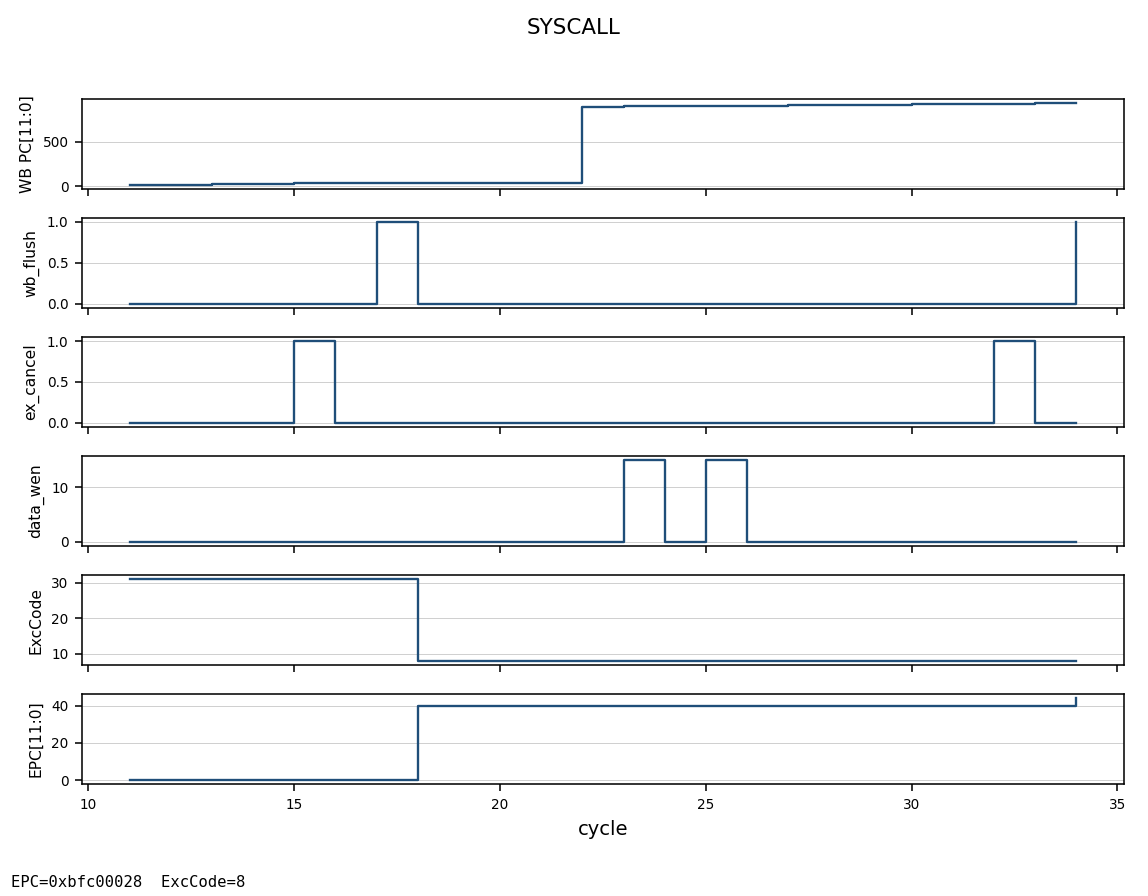
\includegraphics[width=0.92\textwidth]{fig/syscall.png}
\caption{SYSCALL。ExcCode 在清空流水线的下一拍变为 8，EPC 低 12 位为 \texttt{0x028}。}
\end{figure}

溢出是 \texttt{add} 把两个 \texttt{0x80000000} 相加。第 68 拍写回 PC 和下一拍的 EPC 都是 \texttt{0xbfc0004c}，这条 \texttt{add} 的地址；ExcCode 为 12。
BREAK、对地址 1 的 \texttt{lw}、字 \texttt{0xffffffff} 同样在写回当拍对准自己的 PC，ExcCode 为 9、4、10。
五次返回后 \texttt{0x80000000} 起的序号是 1、2、3、4、5，说明 EPC 加 4 都落在异常指令的下一条，没有把异常指令再执行一遍。

\begin{figure}[H]
\centering
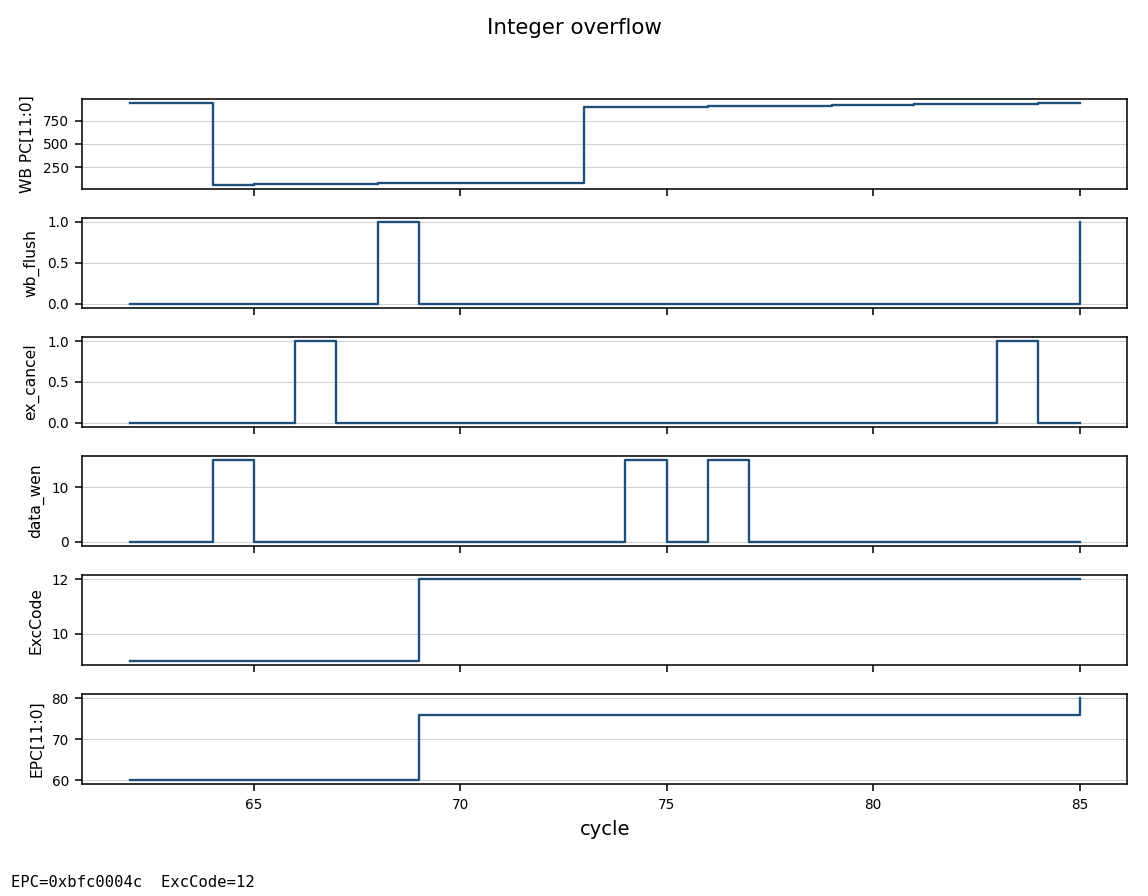
\includegraphics[width=0.92\textwidth]{fig/overflow.png}
\caption{整数溢出。ExcCode 变为 12，EPC 低 12 位为 \texttt{0x04c}。}
\end{figure}

\subsection{三种中断}
软件中断由 \texttt{MTC0} 把 Cause 的位 8 写成 1。Compare 仍是全 1，所以 TI 保持 0。
IP0 要等这拍写入之后才参与 \texttt{int\_req}，因此被打断的不是 \texttt{MTC0} 本身，而是它后面的第一条 \texttt{nop}。
第 152 拍写回 PC 为 \texttt{0xbfc000a0}。下一拍 Cause 为 \texttt{0x00000100}，EPC 也是 \texttt{0xbfc000a0}，Status 为 \texttt{0x0040ff03}：BEV、八位 IM、IE 和 EXL 都为 1。
\texttt{0x100} 只有 IP0，ExcCode 和 BD 都是 0。分支在 \texttt{0xbfc000a8}，这一拍还没有写回。
处理程序清掉 IP0，并把 EPC 改到时钟中断的入口 \texttt{0xbfc000b0}。
第 175 拍 \texttt{ERET} 之后 Cause 为 0，Status 为 \texttt{0x0040ff01}，IE 仍开着，EXL 已清。
\texttt{func\_lab9} 的 \texttt{n82} 把同样的请求留在 \texttt{b 1b} 上，轨迹里的 EPC 等于该分支。
两条路径都是写回级采样，受害指令是当时正要写回的那一条。

\begin{figure}[H]
\centering
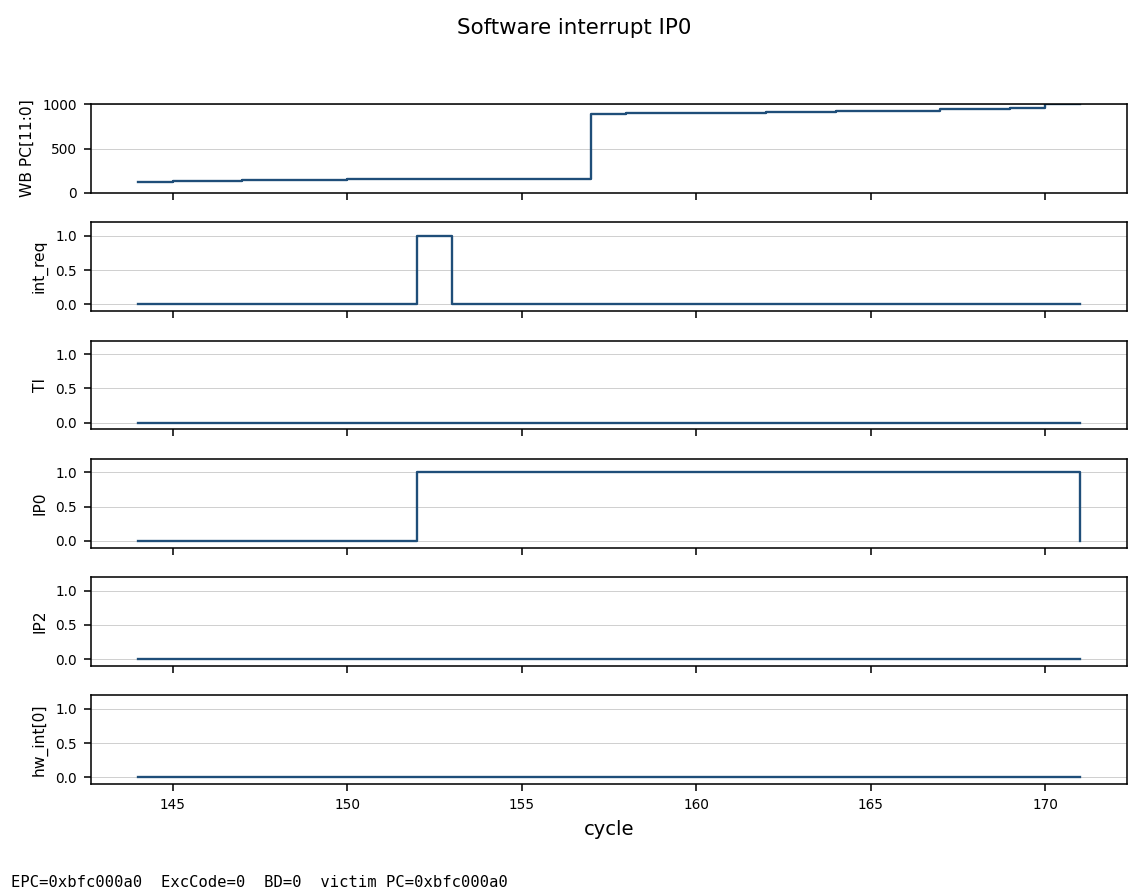
\includegraphics[width=0.92\textwidth]{fig/soft_int.png}
\caption{软件中断。IP0 抬高后 \texttt{int\_req} 出现一拍，写回 PC 转到 \texttt{0xbfc00380}。}
\end{figure}

时钟中断把 Count 清 0、Compare 写成 80，然后执行 \texttt{b 1b; nop}。
TI 先变 1，IP7 和 \texttt{int\_req} 晚一拍。第 342 拍写回的是 \texttt{0xbfc000c8}，即延迟槽里的 \texttt{nop}。
下一拍 Cause 为 \texttt{0xc0008000}：位 31 的 BD 为 1，位 30 的 TI 为 1，IP7 为 1，ExcCode 为 0。
BD 为 1 时 EPC 取受害指令的前一条，所以 EPC 是分支 \texttt{0xbfc000c4}，而不是槽内的 \texttt{nop}。
Status 同时为 \texttt{0x0040ff03}。处理程序把 Compare 写成全 1 来清 TI。
它 \texttt{ERET} 的下一拍 Cause 变成 \texttt{0x80000000}：BD 还留着，TI 和 IP7 已经是 0，EPC 被指到 \texttt{0xbfc000cc}。

\begin{figure}[H]
\centering
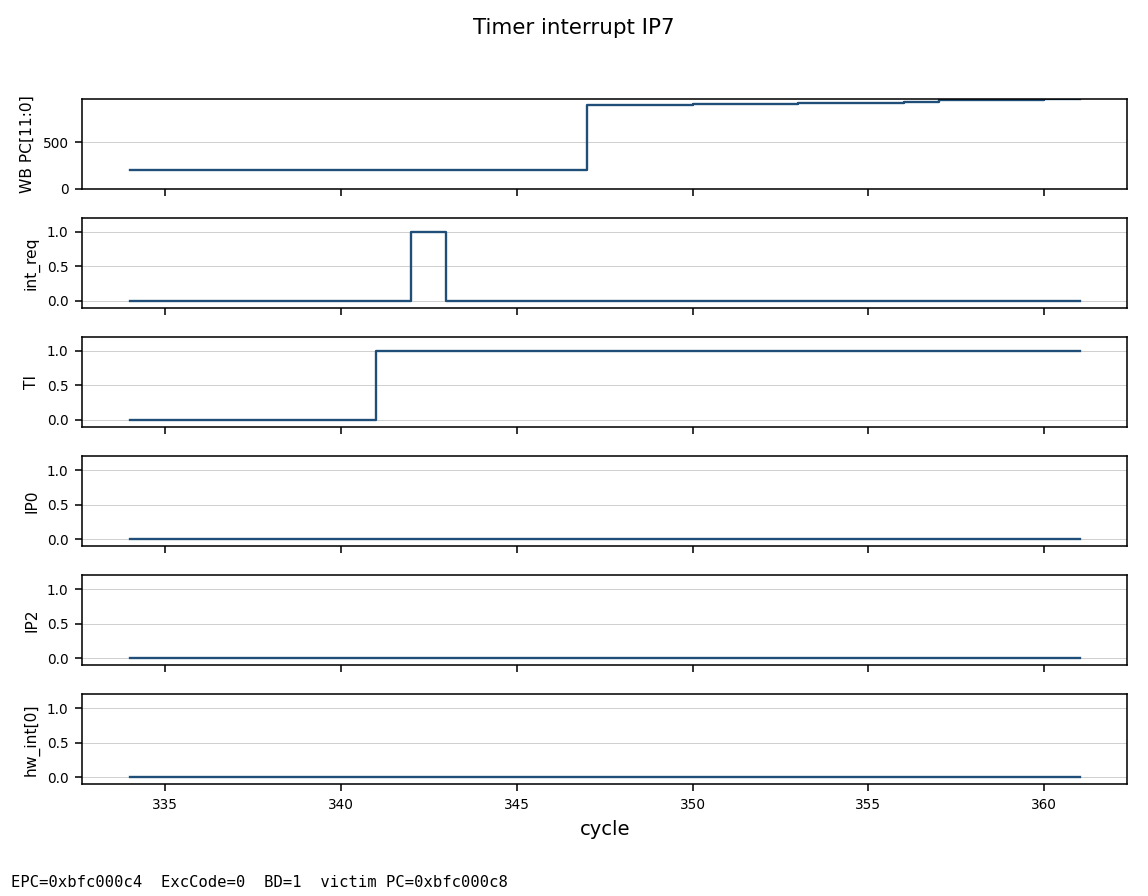
\includegraphics[width=0.92\textwidth]{fig/timer_int.png}
\caption{时钟中断。TI 先于 \texttt{int\_req} 变 1。受害指令在延迟槽，EPC 是前面的分支。}
\end{figure}

\texttt{soc\_lite\_top} 在功能测试里把 \texttt{hw\_int[5:0]} 接成 0，
\texttt{func\_lab9} 因此不会从引脚上进入硬件中断。
定向程序跑到 \texttt{0xbfc000cc} 的分支后，testbench 把 \texttt{hw\_int[0]} 拉高。
IP2 比引脚晚一拍，\texttt{int\_req} 跟着 IP2。第 376 拍写回 PC 就是这条分支。
下一拍 Cause 为 \texttt{0x00000400}，位 10 是 IP2，ExcCode 和 BD 都是 0，因此 EPC 等于受害指令本身 \texttt{0xbfc000cc}。
Status 为 \texttt{0x0040ff03}。处理程序把 Status 写成 \texttt{0x00400000}，IE 关掉，EPC 写成结束循环 \texttt{0xbfc000d4}。
\texttt{ERET} 之后停在这个循环，\texttt{0x80000014} 为 \texttt{0x55}。仿真打印 \texttt{----WAVE PASS!!!----}。

\begin{figure}[H]
\centering
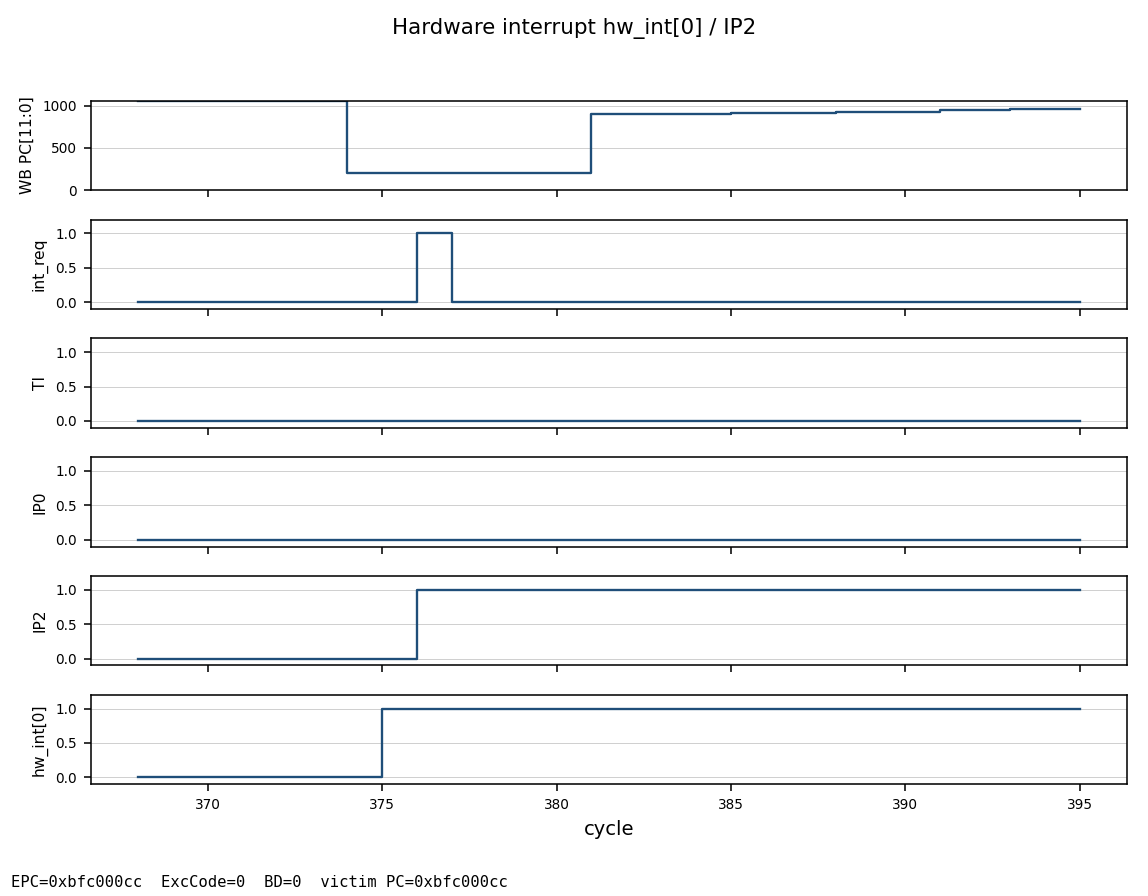
\includegraphics[width=0.92\textwidth]{fig/hw_int.png}
\caption{硬件中断 0。\texttt{hw\_int[0]} 拉高后 IP2 置 1，EPC 为分支 \texttt{0xbfc000cc}。}
\end{figure}

\subsection{记忆游戏}
\label{sec:game}
记忆游戏的源程序在 \texttt{lab3/lab9/memory\_game}。
\texttt{memory\_game()} 先把灯写成 \texttt{0xffff}，用 confreg 计时器做随机种子，然后反复做四件事：
等一次按键，用 \texttt{my\_rand} 产生 8 个图案，把图案显示出来，再读 8 次按键并打分。
每个图案是 1、2、4、8 中的一个。
显示时 \texttt{SOC\_LED} 写成 \texttt{\textasciitilde pattern[i]}，所以图案 8、4、2、1 对应的灯是
\texttt{0xfff7}、\texttt{0xfffb}、\texttt{0xfffd}、\texttt{0xfffe}。
读键时 \texttt{getUserPress} 取 \texttt{SOC\_BTN\_KEY[15:12]} 再把这四位反过来。
扫描到的键码 \texttt{0x1000}、\texttt{0x2000}、\texttt{0x4000}、\texttt{0x8000} 因此读回来是 8、4、2、1。
每采样到一次按键，程序立刻把灯写成 \texttt{\textasciitilde pb}，松开后再写回 \texttt{0xffff}。
\texttt{displayScore} 数 \texttt{pattern[i]==keys[i]} 的个数。
\texttt{SOC\_NUM} 的高字节是已经猜过的次数，低字节是得分；
八次全对时 \texttt{SOC\_LED\_RG1} 写 1，否则写 2，\texttt{SOC\_LED\_RG0} 写 1。

仿真时钟和计时器时钟都是 100\,MHz，\texttt{CPU\_COUNT\_PER\_US} 是 100。
按源程序的毫秒延时，一轮要十几秒仿真时间。
\texttt{confreg} 只在定义了 \texttt{SIM\_FAST\_IO} 时把计时器每次加 5000，并把按键去抖改到 \texttt{key\_count[5]}。
游戏二进制没有改。\texttt{SIM\_FAST\_IO} 只由记忆游戏的仿真脚本定义，\texttt{func\_lab9} 的计时器仍是每拍加 1。
数据 RAM 从 0 开始。\texttt{my\_srand} 在出题前把种子写好，图案和按键都放在栈上。

testbench 先按一次键让游戏进入出题，再按灯的跳变记下 8 个图案，然后用同样的顺序回放。
目标列被扫描到时把按键行拉成 \texttt{0111}，其余列保持松开。
程序按刚读到的键把灯点亮后，testbench 核对这盏灯就是刚才那个图案，再松开，等灯回到 \texttt{0xffff} 后按下一次。

这一轮的图案是 8、8、1、2、8、2、8、2。
八次按键点亮的灯是 \texttt{fff7}、\texttt{fff7}、\texttt{fffe}、\texttt{fffd}、\texttt{fff7}、\texttt{fffd}、\texttt{fff7}、\texttt{fffd}。
低四位里被点亮的那一位正好是图案 8、8、1、2、8、2、8、2，出题的灯和按键点亮的灯逐格相同。

\begin{figure}[H]
\centering
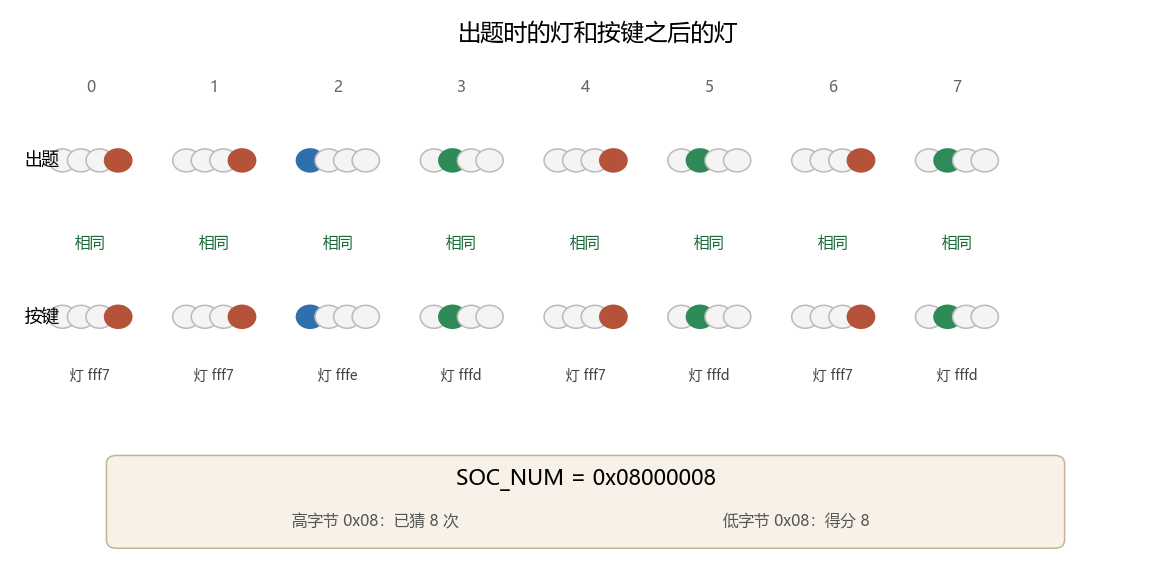
\includegraphics[width=0.92\textwidth]{fig/game_match.png}
\caption{八步里出题时的灯和按键点亮的灯。点亮的圆点是 \texttt{SOC\_LED} 低四位中为 0 的那一位。}
\end{figure}

\texttt{detectKeyPresses} 每读到一次就把 \texttt{SOC\_NUM} 写成猜测次数左移 24 位，八次之后是 \texttt{0x08000000}。
\texttt{displayScore} 再按位或上得分。八格都相同，得分是 8，结果为 \texttt{0x08000008}。
\texttt{led\_rg0} 为 1。得分等于 8 时 \texttt{led\_rg1} 为 1。仿真打印 \texttt{----GAME PASS!!!----}。

出题从第 2 盏灯起，相邻两次亮灯间隔都是 16148 拍。
\texttt{delay(800)} 在计时器每拍加 5000 时要等 \(800\times 100\times 100/5000=16000\) 拍，
多出的 148 拍是写灯和循环本身。第一段间隔是 8132 拍，接近 \texttt{delay(400)} 的 8000 拍。
\texttt{delay} 先写 \texttt{SOC\_TIMER=0}，清零脉冲比紧跟着的第一次读晚几拍。
这一次读到的若仍是上次留下的大数，循环马上结束，清零要到下一次 \texttt{delay} 才起作用。
因此 \texttt{delay(800)} 和 \texttt{delay(400)} 交替成为真正的等待，亮灯间隔就在 16148 拍和 8132 拍之间换。
回放里也能看到同一现象：按下到灯按这个键点亮是 76～112 拍，这是去抖后的列扫描；
灯点亮到下一次按下则在 8076 拍和 60 拍之间交替，8076 拍就是一次完整的 \texttt{delay(400)}。
间隔变短没有改掉读到的键，八次按键点亮的灯仍与出题一致。

\begin{figure}[H]
\centering
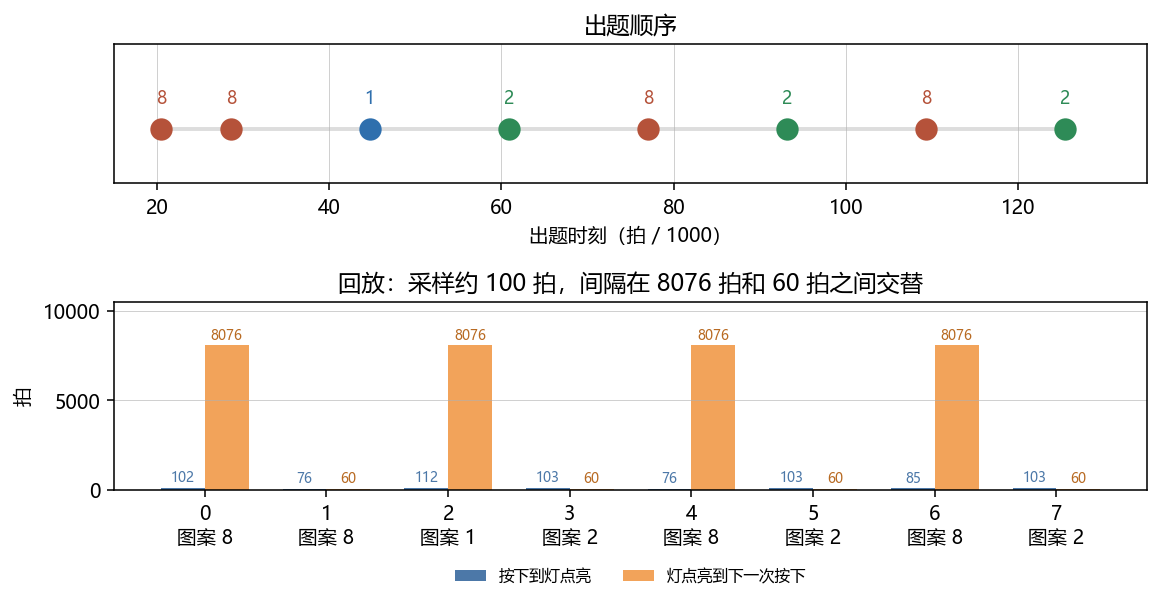
\includegraphics[width=0.92\textwidth]{fig/game_timeline.png}
\caption{出题时刻，以及回放时按下到灯点亮、灯点亮到下一次按下的拍数。}
\end{figure}

实验箱未接，按键和灯都走 confreg 的仿真模型，没有下载比特流。

\section{实验收获}
异常指令一进入执行级，就清掉排在它后面的指令，写回级才把 EXL、EPC 和 ExcCode 写入 CP0。
如果等到写回级才清空流水线，\texttt{SYSCALL} 后面的 \texttt{sw} 会先写进数据 RAM。
\texttt{MFC0} 比 ALU 晚两级才有结果，入口处 \texttt{mfc0} 紧挨 \texttt{bne} 时要按 load-use 停住译码，
写回级再把 CP0 的读数前递出去。
Cause 和 Status 的位域要和参考 CPU 一致：trace 比较的是 \texttt{MFC0} 的整字，
多出来的 TI 或 IP 会在比较中直接报错。
Count 隔拍加 1、IP7 比 TI 晚一拍之后，定时器和软件中断都发生在测试程序的原地循环 \texttt{b 1b} 上。
EPC 等于该分支的 PC，处理程序加 8 后同时跳过这条分支和它的延迟槽。
定向程序里，时钟中断打在延迟槽的 \texttt{nop} 上，BD 为 1，EPC 仍是前面的分支；
硬件中断 0 打在分支本身上，IP2 比 \texttt{hw\_int[0]} 晚一拍。
记忆游戏在仿真里走完一轮：八次按键点亮的灯与出题的灯一致，数码管为 \texttt{0x08000008}，右侧双色灯为 1。

\section{附：源码目录}
CPU 仍在实验1的工程里改。\texttt{lab3} 放测试程序、仿真脚本和本报告。
\begin{itemize}
\item \verb|lab1/lab3/CPU_CDE/mycpu_verify/rtl/myCPU/cp0.v|
\item \verb|lab1/lab3/CPU_CDE/mycpu_verify/rtl/myCPU/IF_stage.v|
\item \verb|lab1/lab3/CPU_CDE/mycpu_verify/rtl/myCPU/ID_stage.v|
\item \verb|lab1/lab3/CPU_CDE/mycpu_verify/rtl/myCPU/EXE_stage.v|
\item \verb|lab1/lab3/CPU_CDE/mycpu_verify/rtl/myCPU/MEM_stage.v|
\item \verb|lab1/lab3/CPU_CDE/mycpu_verify/rtl/myCPU/WB_stage.v|
\item \verb|lab1/lab3/CPU_CDE/mycpu_verify/rtl/myCPU/mycpu.h|
\item \verb|lab1/lab3/CPU_CDE/mycpu_verify/rtl/myCPU/mycpu_top.v|
\item \verb|lab1/lab3/CPU_CDE/cpu132_gettrace/golden_trace.txt|
\item \verb|lab1/lab3/CPU_CDE/soft/func_lab8/obj/inst_ram.coe|
\item \verb|lab1/lab3/CPU_CDE/soft/func_lab9/obj/inst_ram.coe|
\item \verb|lab3/sim/run_gettrace_lab8.tcl|
\item \verb|lab3/sim/run_mycpu_lab8.tcl|
\item \verb|lab3/sim/run_gettrace_lab9.tcl|
\item \verb|lab3/sim/run_mycpu_lab9.tcl|
\item \verb|lab3/sim/wave_tb.v|
\item \verb|lab3/sim/gen_wave_imem.py|
\item \verb|lab3/sim/game_tb.v|
\item \verb|lab3/lab9/memory_game/memory_game/memory_main.c|
\item \verb|lab3/report/report.tex|
\end{itemize}

\end{document}
